\documentclass{standalone}
\usepackage{tikz}
\usetikzlibrary{patterns, positioning}

\begin{document}
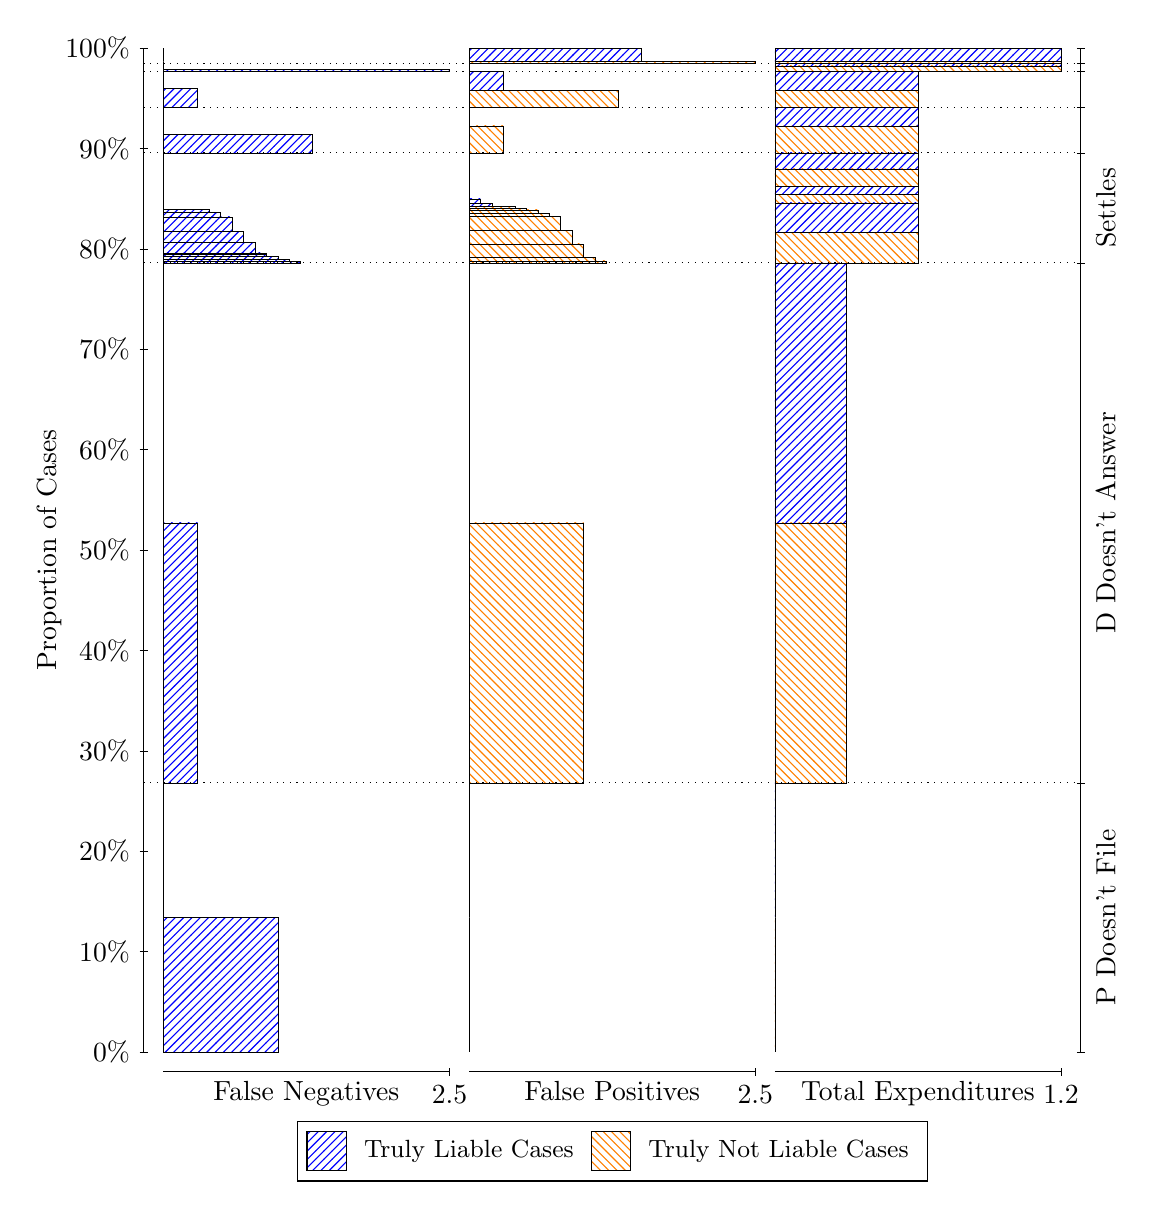
\begin{tikzpicture}
\draw[black, very thin] (1.5,1.75) -- (1.5,14.5);
\node[rotate=90, anchor=center] at (0.3, 8.125) {Proportion of Cases};
\draw[black, very thin] (1.45,1.75) -- (1.55,1.75);
\node[anchor=east] at (1.45, 1.75) {0\%};
\draw[black, very thin] (1.45,3.025) -- (1.55,3.025);
\node[anchor=east] at (1.45, 3.025) {10\%};
\draw[black, very thin] (1.45,4.3) -- (1.55,4.3);
\node[anchor=east] at (1.45, 4.3) {20\%};
\draw[black, very thin] (1.45,5.575) -- (1.55,5.575);
\node[anchor=east] at (1.45, 5.575) {30\%};
\draw[black, very thin] (1.45,6.85) -- (1.55,6.85);
\node[anchor=east] at (1.45, 6.85) {40\%};
\draw[black, very thin] (1.45,8.125) -- (1.55,8.125);
\node[anchor=east] at (1.45, 8.125) {50\%};
\draw[black, very thin] (1.45,9.4) -- (1.55,9.4);
\node[anchor=east] at (1.45, 9.4) {60\%};
\draw[black, very thin] (1.45,10.675) -- (1.55,10.675);
\node[anchor=east] at (1.45, 10.675) {70\%};
\draw[black, very thin] (1.45,11.95) -- (1.55,11.95);
\node[anchor=east] at (1.45, 11.95) {80\%};
\draw[black, very thin] (1.45,13.225) -- (1.55,13.225);
\node[anchor=east] at (1.45, 13.225) {90\%};
\draw[black, very thin] (1.45,14.5) -- (1.55,14.5);
\node[anchor=east] at (1.45, 14.5) {100\%};

\draw[black, very thin] (13.4,1.75) -- (13.4,14.5);
\draw[black, very thin] (13.35,1.75) -- (13.45,1.75);
\node[anchor=west] at (13.35, 1.75) {};
\draw[black, very thin] (13.35,5.1678) -- (13.45,5.1678);
\node[anchor=west] at (13.35, 5.1678) {};
\draw[black, very thin] (13.35,11.771) -- (13.45,11.771);
\node[anchor=west] at (13.35, 11.771) {};
\draw[black, very thin] (13.35,13.169) -- (13.45,13.169);
\node[anchor=west] at (13.35, 13.169) {};
\draw[black, very thin] (13.35,13.748) -- (13.45,13.748);
\node[anchor=west] at (13.35, 13.748) {};
\draw[black, very thin] (13.35,14.202) -- (13.45,14.202);
\node[anchor=west] at (13.35, 14.202) {};
\draw[black, very thin] (13.35,14.3) -- (13.45,14.3);
\node[anchor=west] at (13.35, 14.3) {};
\draw[black, very thin] (13.35,14.5) -- (13.45,14.5);
\node[anchor=west] at (13.35, 14.5) {};

\draw[black, very thin, pattern color=blue, pattern=north east lines] (1.75,1.75) rectangle (3.2033,3.4589);
\draw[black, very thin, pattern color=orange, pattern=north west lines] (1.75,3.4589) rectangle (1.75,5.1678);
\draw[black, very thin, pattern color=blue, pattern=north east lines] (1.75,5.1678) rectangle (2.186,8.4693);
\draw[black, very thin, pattern color=orange, pattern=north west lines] (1.75,8.4693) rectangle (1.75,11.771);
\draw[black, very thin, pattern color=blue, pattern=north east lines] (1.75,11.771) rectangle (3.494,11.795);
\draw[black, very thin, pattern color=blue, pattern=north east lines] (1.75,11.795) rectangle (3.3487,11.814);
\draw[black, very thin, pattern color=blue, pattern=north east lines] (1.75,11.814) rectangle (3.2033,11.851);
\draw[black, very thin, pattern color=blue, pattern=north east lines] (1.75,11.851) rectangle (3.058,11.881);
\draw[black, very thin, pattern color=blue, pattern=north east lines] (1.75,11.881) rectangle (3.058,11.899);
\draw[black, very thin, pattern color=blue, pattern=north east lines] (1.75,11.899) rectangle (2.9127,12.027);
\draw[black, very thin, pattern color=blue, pattern=north east lines] (1.75,12.027) rectangle (2.7673,12.173);
\draw[black, very thin, pattern color=blue, pattern=north east lines] (1.75,12.173) rectangle (2.622,12.356);
\draw[black, very thin, pattern color=blue, pattern=north east lines] (1.75,12.356) rectangle (2.4767,12.415);
\draw[black, very thin, pattern color=blue, pattern=north east lines] (1.75,12.415) rectangle (2.3313,12.454);
\draw[black, very thin, pattern color=orange, pattern=north west lines] (1.75,12.454) rectangle (1.75,13.169);
\draw[black, very thin, pattern color=blue, pattern=north east lines] (1.75,13.169) rectangle (3.6393,13.407);
\draw[black, very thin, pattern color=orange, pattern=north west lines] (1.75,13.407) rectangle (1.75,13.748);
\draw[black, very thin, pattern color=blue, pattern=north east lines] (1.75,13.748) rectangle (2.186,13.991);
\draw[black, very thin, pattern color=orange, pattern=north west lines] (1.75,13.991) rectangle (1.75,14.202);
\draw[black, very thin, pattern color=blue, pattern=north east lines] (1.75,14.202) rectangle (5.3833,14.23);
\draw[black, very thin, pattern color=orange, pattern=north west lines] (1.75,14.23) rectangle (1.75,14.3);
\draw[black, very thin, pattern color=orange, pattern=north west lines] (1.75,14.3) rectangle (1.75,14.328);
\draw[black, very thin, pattern color=blue, pattern=north east lines] (1.75,14.328) rectangle (1.75,14.5);
\draw[black, very thin, pattern color=orange, pattern=north west lines] (5.6333,1.75) rectangle (5.6333,3.4589);
\draw[black, very thin, pattern color=blue, pattern=north east lines] (5.6333,3.4589) rectangle (5.6333,5.1678);
\draw[black, very thin, pattern color=orange, pattern=north west lines] (5.6333,5.1678) rectangle (7.0867,8.4693);
\draw[black, very thin, pattern color=blue, pattern=north east lines] (5.6333,8.4693) rectangle (5.6333,11.771);
\draw[black, very thin, pattern color=orange, pattern=north west lines] (5.6333,11.771) rectangle (7.3773,11.798);
\draw[black, very thin, pattern color=orange, pattern=north west lines] (5.6333,11.798) rectangle (7.232,11.843);
\draw[black, very thin, pattern color=orange, pattern=north west lines] (5.6333,11.843) rectangle (7.0867,12.014);
\draw[black, very thin, pattern color=orange, pattern=north west lines] (5.6333,12.014) rectangle (6.9413,12.185);
\draw[black, very thin, pattern color=orange, pattern=north west lines] (5.6333,12.185) rectangle (6.796,12.361);
\draw[black, very thin, pattern color=orange, pattern=north west lines] (5.6333,12.361) rectangle (6.6507,12.404);
\draw[black, very thin, pattern color=orange, pattern=north west lines] (5.6333,12.404) rectangle (6.5053,12.444);
\draw[black, very thin, pattern color=orange, pattern=north west lines] (5.6333,12.444) rectangle (6.36,12.464);
\draw[black, very thin, pattern color=orange, pattern=north west lines] (5.6333,12.464) rectangle (6.2147,12.485);
\draw[black, very thin, pattern color=blue, pattern=north east lines] (5.6333,12.485) rectangle (5.924,12.525);
\draw[black, very thin, pattern color=blue, pattern=north east lines] (5.6333,12.525) rectangle (5.7787,12.584);
\draw[black, very thin, pattern color=blue, pattern=north east lines] (5.6333,12.584) rectangle (5.6333,13.169);
\draw[black, very thin, pattern color=orange, pattern=north west lines] (5.6333,13.169) rectangle (6.0693,13.51);
\draw[black, very thin, pattern color=blue, pattern=north east lines] (5.6333,13.51) rectangle (5.6333,13.748);
\draw[black, very thin, pattern color=orange, pattern=north west lines] (5.6333,13.748) rectangle (7.5227,13.959);
\draw[black, very thin, pattern color=blue, pattern=north east lines] (5.6333,13.959) rectangle (6.0693,14.202);
\draw[black, very thin, pattern color=orange, pattern=north west lines] (5.6333,14.202) rectangle (5.6333,14.272);
\draw[black, very thin, pattern color=blue, pattern=north east lines] (5.6333,14.272) rectangle (5.6333,14.3);
\draw[black, very thin, pattern color=orange, pattern=north west lines] (5.6333,14.3) rectangle (9.2667,14.328);
\draw[black, very thin, pattern color=blue, pattern=north east lines] (5.6333,14.328) rectangle (7.8133,14.5);
\draw[black, very thin, pattern color=orange, pattern=north west lines] (9.5167,1.75) rectangle (9.5167,3.4589);
\draw[black, very thin, pattern color=blue, pattern=north east lines] (9.5167,3.4589) rectangle (9.5167,5.1678);
\draw[black, very thin, pattern color=orange, pattern=north west lines] (9.5167,5.1678) rectangle (10.425,8.4693);
\draw[black, very thin, pattern color=blue, pattern=north east lines] (9.5167,8.4693) rectangle (10.425,11.771);
\draw[black, very thin, pattern color=orange, pattern=north west lines] (9.5167,11.771) rectangle (11.333,12.163);
\draw[black, very thin, pattern color=blue, pattern=north east lines] (9.5167,12.163) rectangle (11.333,12.532);
\draw[black, very thin, pattern color=orange, pattern=north west lines] (9.5167,12.532) rectangle (11.333,12.637);
\draw[black, very thin, pattern color=blue, pattern=north east lines] (9.5167,12.637) rectangle (11.333,12.747);
\draw[black, very thin, pattern color=orange, pattern=north west lines] (9.5167,12.747) rectangle (11.333,12.965);
\draw[black, very thin, pattern color=blue, pattern=north east lines] (9.5167,12.965) rectangle (11.333,13.169);
\draw[black, very thin, pattern color=orange, pattern=north west lines] (9.5167,13.169) rectangle (11.333,13.51);
\draw[black, very thin, pattern color=blue, pattern=north east lines] (9.5167,13.51) rectangle (11.333,13.748);
\draw[black, very thin, pattern color=orange, pattern=north west lines] (9.5167,13.748) rectangle (11.333,13.959);
\draw[black, very thin, pattern color=blue, pattern=north east lines] (9.5167,13.959) rectangle (11.333,14.202);
\draw[black, very thin, pattern color=orange, pattern=north west lines] (9.5167,14.202) rectangle (13.15,14.272);
\draw[black, very thin, pattern color=blue, pattern=north east lines] (9.5167,14.272) rectangle (13.15,14.3);
\draw[black, very thin, pattern color=orange, pattern=north west lines] (9.5167,14.3) rectangle (13.15,14.328);
\draw[black, very thin, pattern color=blue, pattern=north east lines] (9.5167,14.328) rectangle (13.15,14.5);
\draw[black, dotted] (1.5,5.1678) -- (13.4,5.1678);
\draw[black, dotted] (1.5,11.771) -- (13.4,11.771);
\draw[black, dotted] (1.5,13.169) -- (13.4,13.169);
\draw[black, dotted] (1.5,13.748) -- (13.4,13.748);
\draw[black, dotted] (1.5,14.202) -- (13.4,14.202);
\draw[black, dotted] (1.5,14.3) -- (13.4,14.3);
\draw[black, very thin] (1.75,1.5) -- (5.3833,1.5);
\node[anchor=north] at (3.5667, 1.5) {False Negatives};
\draw[black, very thin] (5.3833,1.45) -- (5.3833,1.55);
\node[anchor=north] at (5.3833, 1.45) {2.5};

\draw[black, very thin] (5.6333,1.5) -- (9.2667,1.5);
\node[anchor=north] at (7.45, 1.5) {False Positives};
\draw[black, very thin] (9.2667,1.45) -- (9.2667,1.55);
\node[anchor=north] at (9.2667, 1.45) {2.5};

\draw[black, very thin] (9.5167,1.5) -- (13.15,1.5);
\node[anchor=north] at (11.333, 1.5) {Total Expenditures};
\draw[black, very thin] (13.15,1.45) -- (13.15,1.55);
\node[anchor=north] at (13.15, 1.45) {1.2};

\node[black, centered, rotate=90] at (13.72, 3.4589) {P Doesn't File};
\node[black, centered, rotate=90] at (13.72, 8.4693) {D Doesn't Answer};
\node[black, centered, rotate=90] at (13.72, 12.47) {Settles};





\draw (7.449999999999999,1.5) node[draw=none] (baseCoordinate) {};
\begin{scope}[align=center]
        \matrix[scale=0.5, draw=black, below=0.5cm of baseCoordinate, nodes={draw}, column sep=0.1cm]{
            \node[rectangle, draw, minimum width=0.5cm, minimum height=0.5cm, pattern=north east lines, pattern color=blue] {}; &
            \node[draw=none, font=\small] (B) {Truly Liable Cases}; &
            \node[rectangle, draw, minimum width=0.5cm, minimum height=0.5cm, pattern=north west lines, pattern color=orange] {}; &
            \node[draw=none, font=\small] (B) {Truly Not Liable Cases}; \\
            };
\end{scope}

\end{tikzpicture}
\end{document}